\documentclass[a4paper, 12pt]{article}
\usepackage[top=2cm, bottom=2cm, left=2.5cm, right=2.5cm]{geometry}
\usepackage[utf8]{inputenc}
\usepackage[brazilian]{babel}
\usepackage{indentfirst}
\usepackage{graphicx}
\usepackage{wrapfig}
\usepackage[pdftex]{hyperref}
\usepackage{amssymb} 
\graphicspath{ {imagens/} }

\begin{document}
%
\begin{titlepage} %iniciando a "capa"
	\begin{center} %centralizar o texto abaixo
		{\large Unicamp}\\[0.2cm] %0,2cm é a distância entre o texto dessa linha e o texto da próxima
		{\large [Estatística]}\\[0.2cm] % o comando \\ "manda" o texto ir para próxima linha
		{\large [Samara F. Kiihl]}\\[3.2cm]
		{\bf \huge Estatística}\\[0.2cm] 
		{\bf \large para experimentalistas}\\[4.9cm]
		% o comando \bf deixa o texto entre chaves em negrito. O comando \huge deixa o texto enorme
	\end{center} %término do comando centralizar
	{\large Erik Yuji Goto}\\[10cm] % o comando \large deixa o texto grande
	\begin{center}
		{\large Campinas}\\[0.2cm]
		{\large 2021}
	\end{center}
\end{titlepage} %término da "capa"


\tableofcontents
\newpage

\section{Estatística Descritiva}
	São métodos para resumir e descrever os dados.
	
	É o primeiro passo antes de qualquer análise estatística. O resumo dos dados pode ser feito por:
	\begin{itemize}
		\item Métricas quantitativas: média, mediana, desvio padrão, proporções;
		\item Ferramentas visuais: gráfico.
	\end{itemize}
 
	\paragraph{Estrutura básica de dados - Variável:}
	\begin{itemize}
		\item Qualitativa
			\begin{itemize}
				\item Nominal: Não existe ordenação. Ex: sexo, estado civil, profissão;
				\item Ordinal: Existe uma certa ordem. Ex: escolaridade, estágio da doença, classe social.
			\end{itemize}
		\item Quantitativa
			\begin{itemize}
				\item Discreta: Os valores possíveis formam um conjunto finito ou enumerável. Ex: nº filhos, nº ovos de páscoa;
				\item Contínua: Os valores possíveis estão dentro de um intervalo dos números reais. Ex: peso, altura, salário.
			\end{itemize}
	\end{itemize}
	
\subsection{Medidas Resumo(estatísticas sumárias)}
	O \textbf{objetivo} é resumir os dados, através de valores que representem o conjunto de dados em relação à alguma característica.
\subsubsection{Média Aritmética}
	\begin{center}
		\LARGE
		$\overline{x} = \frac{1}{n} \sum_{i = 1}^{n} x_{i}$
	\end{center}
\subsubsection{Mediana}
	Valor que separa os dados em dois grupos de tamanhos iguais, ou seja, 50\% das observações em cada, de acordo com \textbf{seus valores ordenados}.
	
	Para n ímpar e para n par respectivamente:
	\begin{center}
		\LARGE
		$
		Q_{2} = x_{(\frac{n+1}{2})}
		$
		
		$
		Q_{2} = \frac{x_{(\frac{n}{2})} + x_{(\frac{n}{2} + 1)}}{2}
		$
	\end{center}

\subsubsection{Moda}
	É o valor com maior número de ocorrência nos dados.
	
	A moda não precisa ser única

	\begin{center}
		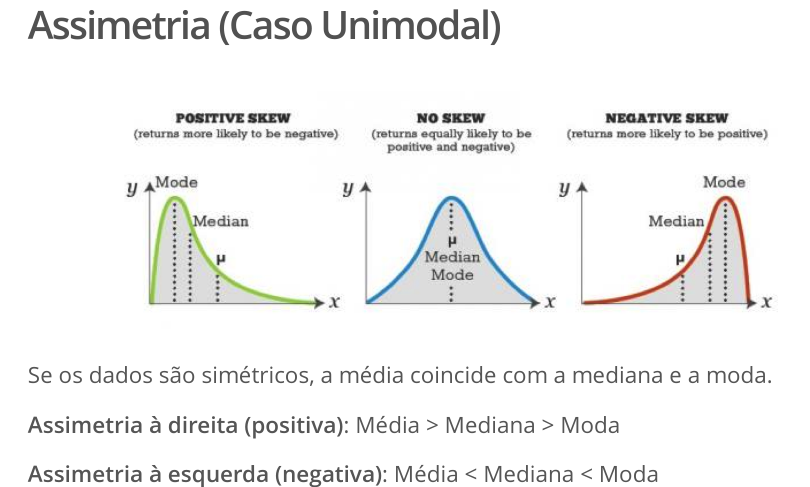
\includegraphics[width=0.7\linewidth]{imagens/moda.png}
	\end{center}
\subsubsection{Desvio}
	O desvio de uma observação $x_{i}$ da média $\overline{x}$ é a diferença entre a observação e a média dos dados.
	A média dos desvios ao quadrado é denominada \textbf{variância}:
	\begin{center}
		\LARGE
		$
		s^{2} = \frac{1}{n-1}\sum_{i = 1}^{n}(x_{i} - \overline{x})^{2}
		$
	\end{center}
	Desvio padrão é a raiz quadrada da variância:
	\begin{center}
		\LARGE
		$
		s = \sqrt{\frac{1}{n-1}\sum_{i = 1}^{n}(x_{i} - \overline{x})^{2}}
		$
	\end{center}
	
\subsubsection{Coeficiente de Variação}
	É a razão do desvio padrão \textbf{s} pela média $\overline{x}$
	\begin{center}
		\LARGE
		$
		c_{v} = \frac{s}{\overline{x}}
		$
	\end{center}

\subsection{Quartis}
	Consiste em dividir os dados em 4 partes iguais.
	Para se obter os quartis:
	\begin{enumerate}
		\item Ordene os dados em ordem crescente;
		\item Encontre a mediana $Q_{2}$;
		\item Considere o subconjunto de dados abaixo da mediana. $Q_{1}$ é a mediana deste subconjunto de dados;
		\item Considere o subconjunto de dados acima da mediana. $Q_{3}$ é a mediana deste subconjunto.
	\end{enumerate}
	\begin{center}
		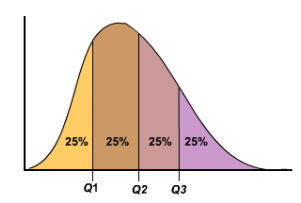
\includegraphics[width=0.5\linewidth]{imagens/quartis.png}
	\end{center}
	Para uma relação simétrica(ou quase), temos as seguintes relações:
	\begin{center}
		$Q_{2} - x_{(1)} \approx x_{n} - Q_{2}$
		
		$Q_{2} - Q_{1} \approx Q_{3}-Q_{2}$
		
		$Q_{1} - x_{1} \approx x_{n}-Q_{3}$
	\end{center}
	\begin{flushright}
		\textit{$x_{1}$ é o minimo\\
		$x_{n}$ é o máximo}
	\end{flushright}
	Distância entre as medianas e $Q_{1}, Q_{3}$ menores que as distâncias entre os extremos $Q_{1} e Q_{3}$

\subsubsection{Intervalo Interquartílico}
	A vantagem do uso de quartis sobre o desvio padrão é que os quartis são mais resistentes a dados extremos, são mais robustos.
	O intervalo quartílico representa 50\% dos dados localizados na parte central da distribuição.
	\begin{center}
		\LARGE
		$IQ = Q_{3} - Q_{1}$
	\end{center}
	\begin{center}
		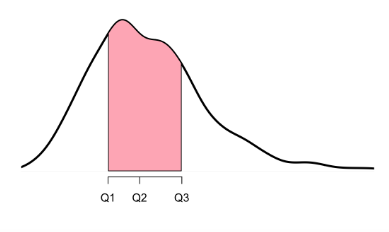
\includegraphics[width=0.4\linewidth]{imagens/iq.png}
	\end{center}
	
\subsubsection{Esquema dos 5 números e Boxplot}
	\begin{center}
		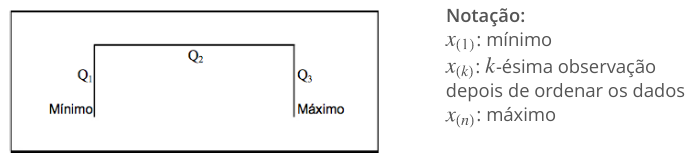
\includegraphics[width=0.7\linewidth]{imagens/esquema}
	\end{center}
	
	\textbf{Dados discrepantes(outliers):} Como regra geral, dizemos que uma obsevação é uma potencial outlier se está:
		\begin{center}
			Abaixo de $Q_{1} - 1,5.IQ$\\
			Acima de $Q_{3} + 1,5.IQ$
		\end{center}
		
	O \textbf{boxplot} é a representação gráfica do esquema dos 5 números.
	\begin{center}
		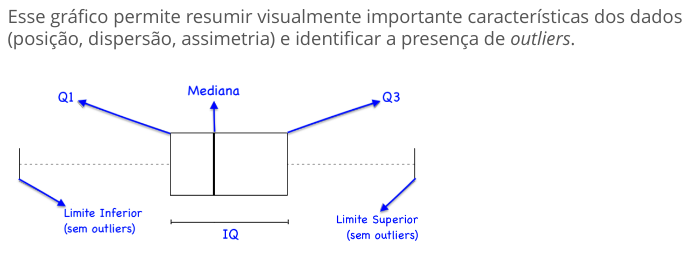
\includegraphics[width=0.9\linewidth]{imagens/boxplot}
	\end{center}
	Para descobrir os limites superior e inferior usamos a fórmula para encontrar os \textit{outliers}. 
	
\subsection{Análise Descritiva Bivariada}
\subsubsection{Coeficiente de Correlação}
	É uma medida resumo que representa associação linear entre duas variáveis quantitativas.
	
	Dado n pares de observações $(x_{1}, y_{1}), (x_{2}, y_{2}) ... (x_{n}, y_{n})$
	\begin{center}
		\LARGE
		$Corr(X, Y) = \frac{1}{n-1} \sum_{i = 1}^{n} (\frac{x_{i} - \overline{x}}{s_{x}})(\frac{y_{i} - \overline{y}}{s_{y}})$
		\normalsize
		
		$-1\leq Corr(X,Y) \leq 1$
	\end{center}
	Onde $ s_{x} e s_{y}$ são os desvios padrões de X e Y.
	
	\textbf{Corr(X,Y) próximo de 1:} X e Y estão positivamente associados e o tipo de associação entre as variáveis é linear.
	
	\textbf{Corr(X,Y) próximo de 0:} X e Y não estão correlacionados.
	
	\textit{Atenção:} Correlação não implica causa
	
\section{Probabilidade}
	\textbf{Espaço amostral:} Todos os resultados possíveis do experimento, denotado por \\$\Omega = \{w_{1},w_{2},...\}$.
	
	\textbf{Evento:} Dizemos que o evento A ocorreu sempre que o resultado observado pertencer ao subconjunto de elementos do evento A.
	
\subsubsection{Probabilidade de União de Eventos}
	\begin{center}
		\LARGE
		$P(A\cup B) = P(A) + P(B) - P(A\cap B)$
	\end{center}
	\begin{center}
		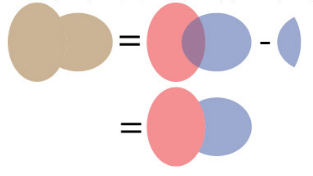
\includegraphics[width=0.5\linewidth]{imagens/prob}
	\end{center}
	
\subsubsection{Evento Complementar}
	Sejam A e B subconjuntos de $\Omega$. Eles são complementares se $A\cap B= \phi$ e $A\cup B = \Omega$.
	
	Como $P(A) + P(B) = 1$, então $P(B) = 1 - P(A)$.

\subsection{Regras de Contagem}
\subsubsection{Regra da adição}
	Suponha que temos dois procedimentos possíveis para executarmos uma tarefa, ou seja, basta executarmos um dos procedimentos para que a tarefa tenha sido executada.
	
	O total de maneiras para executarmos a tarefa é $n_{1} + n_{2}$.
	
\subsection{Regra da multiplicação}
	Suponha que para realizarmos uma tarefa temos que executar dois procedimentos, denotados $p_{1} e p_{2}$.
	
	O total de maneiras para executarmos a tarefa é dado por $p_{1}*p_{2}$.
	
\subsection{Permutação}
	Suponha que temos \textit{n} caixas e queremos dispor os \textit{n} objetos nessas caixas. 
	
	Aplicando a regra da multiplicação, temos que o número de maneiras de permutar n é: $n!$
	
\subsection{Arranjo}
	O número de maneiras de arranjar n elementos em r caixas é:
	\begin{center}
		\LARGE
		$A(n ,r) = \frac{n!}{(n-r)!}$
	\end{center}
	
\subsection{Combinação}
	A combinação é semelhante ao arranjo, com exceção de que a ordem não importa:
	\begin{center}
		\LARGE
		$C(n, r) = {n\choose r} = \frac{n!}{r!(n-r)!}$
	\end{center}
	
\subsection{Probabilidade Condicional}
	Encontrar a probabilidade de um evento quando você tem alguma outra informação sobre o evento.
	
	A probabilidade condicional de \textbf{B} dado \textbf{A} é expressa por $P(B\mid A)$.
	
	Supondo que o resultado do experimento esteja contido no evento A.
	
	\begin{center}
		\LARGE
		$P(B\mid A) = \frac{P(A\cap B)}{P(A)}$
	\end{center}	
	
\subsection{Independência}
	Quando $P(B\mid A) = P(B)$, informação sobre A \textit{não altera} a probabilidade do evento B, dizemos que A e B são \textbf{independentes}.
	\begin{center}
		\LARGE
		$P(A\cap B) = P(A)P(B)$
	\end{center}

\subsection{Teorema das Probabilidades Totais}
	A probabilidade do evento A é uma média ponderada de $P(A\mid B)$ e $P(A\mid B^{c})$. O peso de cada probabilidade condicional é a probabilidade do evento que está sendo levado em conta ao calcular a probabilidade condicional de A.
	\begin{center}
		\LARGE
		$P(A) = P(A\mid B)P(B) + P(A\mid B^{c})P(B^{c})$
	\end{center}

\subsection{Teorema de Bayes}
	\begin{center}
		\LARGE
		$P(B_{i}\mid A) = 
		\frac{P(A\mid B_{i})P(B_{i}) }{\sum_{i = 1}^{n} P(A\mid B_{i})P(B_{i})}
		$
	\end{center}

\section{Variável Aleatória}
	Uma função X que associa a cada elemento do espaço amostral um valor num conjunto enumerável de pontos da reta é denominada \textit{variável aleatória discreta}.
	\begin{center}
		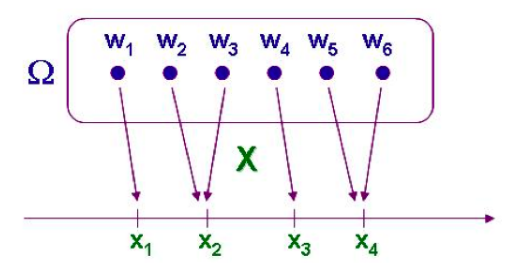
\includegraphics[width=0.5\linewidth]{imagens/vardis}
	\end{center}
	
\subsection{Distribuição de probabilidade}
	Associa uma probabilidade $P(X = x)$ para cada valor possível, x, da variável aleatória X.
	\begin{center}
		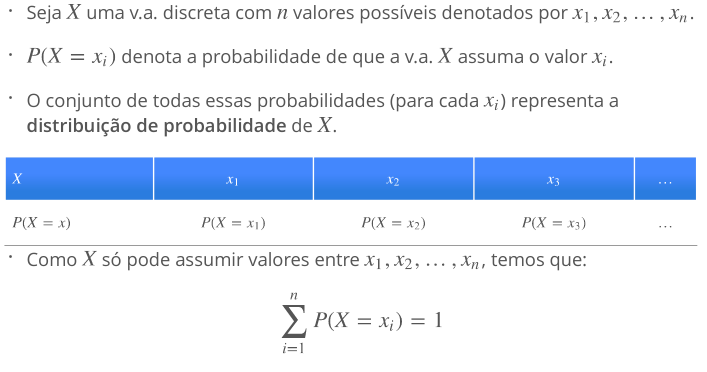
\includegraphics[width=0.8\linewidth]{imagens/vardis3}
	\end{center}

\subsection{Função de Distribuição Acumulada}
	É definida por
	\begin{center}
		\LARGE
		$F(x) = P(X \leq x), x \in \Re $
	\end{center}
	Exemplo:
	\begin{center}
		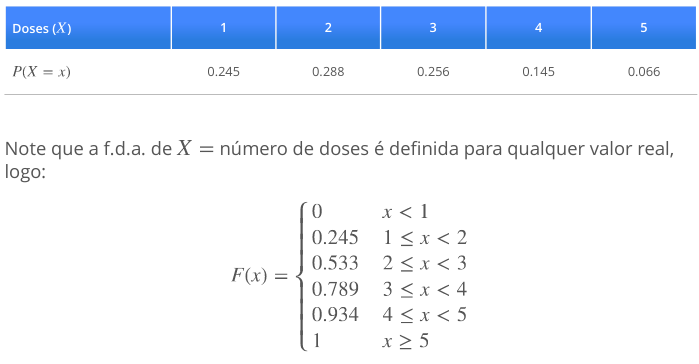
\includegraphics[width=0.8\linewidth]{imagens/vardis2}
	\end{center}

\subsection{Esperança}
	A esperança(ou valor esperado) da variável X é dada por:
	\begin{center}
		$E(X) = \mu = \sum_{i = 1}^{n} x_{i}P(X = x_{i})$
	\end{center}

	Não podemos interpretar E(X) como o valor que esperamos que X irá assumir, mas sim como uma \textbf{média} dos valores observados de X ao longo de muitas repetições do experimento aleatório.
	
	\textbf{Propriedades da Esperança}
	\begin{enumerate}
		\item Para qualquer v.a. X e constantes a e b: \\ $E(aX + b) = aE(X) + b$
		\item $E(\sum_{i=1}^{n} X_{i}) = \sum_{i=1}^{n}E(X_{i})$
		\item Esperança de uma funçao de uma variável aleatória - útil na hora de calcular a variância:\\
		$E[g(X)] = \sum_{i}g(x_{i})p(x_{i})$
	\end{enumerate}
\subsection{Variância}
	Queremos uma medida para quantificar quão distantes os valores da v.a. X estão da sua esperança. A variância é calculada por:
	\begin{center}
		\LARGE
		$Var(X) = E(x^{2}) - [E(X)]^{2}$
	\end{center}
	
	\textbf{Propriedades da Variância}
	\begin{enumerate}
		\item Para qualquer v.a. X e ctes a e b:\\$Var(aX + b) = a^{2}Var(X)$
		\item Se $x_{1}, x_{2}, ... x_{n}$ são variáveis aleatórias independentes:\\
		$Var(\sum_{i=1}^{n}X_{i}) = \sum_{i=1}^{n}Var(X_{i})$
	\end{enumerate}

\subsection{Mediana e Moda}
	Sabemos que a média é encontrada pela esperança.
	
	A \textit{mediana(Md)} é o valor que satisfaz:
	\begin{center}
		\LARGE
		$P(X\geq Md) \geq \frac{1}{2}$ e $P(X\leq Md) \geq \frac{1}{2}$
	\end{center}

	A \textit{moda(Mo)} é o valor da variável X com maior probabilidade de ocorrência.
	\begin{center}
		\LARGE
		$P(X = M_{o}) = max\{p_{1}, p_{2}, ...\}$
	\end{center}

\subsection{Principais Modelos Discretos}
\subsubsection{Uniforme Discreta}
	Ocorre se cada valor possível tem a mesma probabilidade de ocorrer. Exemplo: Lançamento de um dado.
	\begin{center}
		\LARGE
		$P(X=x_{i}) = \frac{1}{k}$ 
	\end{center}
	\textbf{Notação:} $X\sim$ Uniforme Discreta$\{1, 2, ...\}$
	
\subsubsection{Bernoulli}
	Quando cada observação de um experimento aleatório é \textbf{binária}, tem apenas dois resultados possíveis:
	\begin{itemize}
		\item Sucesso;
		\item Fracasso.
	\end{itemize}
	Seja X assumindo apenas valores 0 e 1, onde X= 1 corresponde a sucesso e seja p a probabilidade de sucesso
	\begin{center}
		\LARGE
		$P(X = x) = p$ , se x = 1\\
		$P(X = x) = 1 - p$ , se x = 0
	\end{center}
	Ou de forma equivalente:
	\begin{center}
		\LARGE
		$P(X = x) = p^{x}(1-p)^{1-x}$ , para x = 0,1
	\end{center}
	\textbf{Notação:} $X \sim b(p)$
	
	Além disso, calculamos a \textbf{esperança} e a \textbf{variância} como sendo
	\begin{center}
		\LARGE
		$E(x) = p$\\ $Var(X) = p(1-p)$
	\end{center}
	
\subsubsection{Modelo Binomial}
	Três condições para ser usado:
	\begin{enumerate}
		\item \textbf{n} ensaios de Bernoulli;
		\item Os ensaios são independentes;
		\item A probabilidade de sucesso \textbf{p} é a mesma em todo o ensaio.
	\end{enumerate}	
	
	\textbf{Notação:} $X \sim Bin(n,p)$
		
	A probabilidade de se observar x é dada pela expressão geral:	
	\begin{center}
		\LARGE
		$p(X = x) = {n \choose x}p^{x}(1-p)^{n-x}$, x = 0, 1, ... n
	\end{center}
	A \textbf{esperança} e \textbf{variância} de uma v.a. Binomial são dados por:
	\begin{center}
		\LARGE
		$E(X) = np$\\
		$Var(X) = np(1-p)$
	\end{center}
	
\subsubsection{Distribuição Geométrica}
	Seja X a v.a. que representa o número de ensaios de Bernoulli até a ocorrência do primeiro sucesso. Então dizemos que X segue uma distribuição \textbf{Geométrica} com parâmetro p.
	
	\textbf{Notação:} $X\sim G(p)$	
	
	A probabilidade de se observar x é:
	\begin{center}
		\LARGE
		$P(X = x) = (1-p)^{x-1}p$ , x = 1, 2, ...
	\end{center}
	A esperança e variância são
	\begin{center}
		\LARGE
		$E(X) = \frac{1}{p}$\\ $Var(X) = \frac{1-p}{p^{2}}$
	\end{center}
	A função de distribuição acumulada de uma v.a. G(p) é dada por:
	\begin{center}
		\LARGE
		$F(x) = P(X\leq x) = 1-(1-p)^{x}$
	\end{center}
	\textbf{Propriedade de perda de Memória:} O fato de já termos observado \textit{m} fracassos sucessivos não muda a probabilidade do número de ensaios até o primeiro sucesso ocorrer.

\subsubsection{Hipergeométrica}
	\begin{itemize}
		\item População dividida em duas características;
		\item Extração casuais \textbf{sem reposição}.
	\end{itemize}
	
	O que queremos resolver:
	\begin{itemize}
		\item N objetos;
		\item r têm a característica A;
		\item N-r têm a característica B;
		\item Um grupo de n elementos é escolhido ao acaso, dentre os N possíveis, sem reposição.
	\end{itemize}
	
	\textit{Objetivo} é calcular a probabilidade de que este grupo de n elementos contenha x elementos com característica A.
	
	\textbf{Notação:} $X\sim Hip(N, n, r)$ \\
	N = tamanho da população\\ n = tamanho da amostra\\ r = número de indivíduos com a característica(em relação à população total)
	
	A probabilidade de se observar x é dada por:
	\begin{center}
		$P(X = x) = \frac{{r \choose x} {N-r \choose n-x}}{{N \choose n}} $ , $0\leq x\leq min\{r, n\}$
	\end{center}
	
	\textbf{Esperança e Variância}
	\begin{center}
		\LARGE
		$E(X) = \frac{nr}{N}$
		
		$Var(X) = \frac{nr}{N}(1 - \frac{r}{N})\frac{(N-n)}{(N-1)}$ 
	\end{center}
	
\subsubsection{Distribuição de Poisson}	
	Muitas vezes, em problemas em que seria natural usar a distribuição binomial, temos \textbf{n} muito grande e p muito pequeno. Nestes casos podemos usar o teorema de Poisson:
	\begin{center}
		\LARGE
		$P(X = x) \approx \frac{e^{-np} (np)^{x}}{x!}$ , x = 0, 1, 2...
	\end{center}
	
	Considera-se o critério $np \leq 7$ para usar essa aproximação.
	
	Outra regra prática: $n \geq 20$ e $p \leq 0,05$
	
	Uma variável aleatória x tem distribuição de Poisson com parâmetro $\lambda > 0$, se sua função de probabilidade é dada por:
	\begin{center}
		\LARGE
		$P(X = x) = \frac{e^{- \lambda} \lambda ^{x}}{x!}$ , x = 0, 1, 2, ...
	\end{center}
	
	$\lambda$ é chamado de taxa de ocorrência\\
	\textbf{Notação:} $X \sim P(\lambda)$
	\begin{center}
		\LARGE
		$E(X) = Var(X) = \lambda$
	\end{center}
	
\newpage
\section{Variáveis Aleatórias Contínuas}
Variável Aleatória com valores possíveis em um intervalo no conjunto de números reais.
	
	\begin{figure}[h]
		\centering
		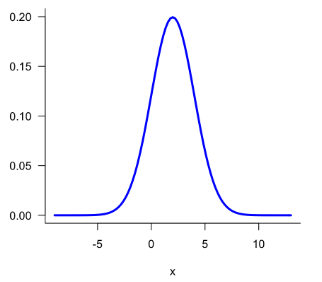
\includegraphics[width=0.5\linewidth]{imagens/vac}
		\caption{$\int_{-\infty}^{\infty} f(x)dx = 1$}
		\label{fig:vac}
	\end{figure}
	
	A probabilidade de que uma v.a. x contínua pertença a um intervalo da reta (a, b], $a < b$ é:
	
	\begin{center}
		\Large
		$
		P(a<x<b) = \int_{a}^{b} f(x)dx
		$
	\end{center}
	\begin{figure}[h]
		\centering
		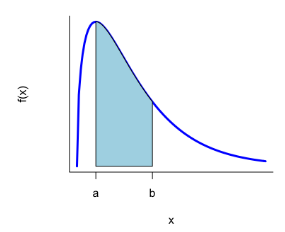
\includegraphics[width=0.5\linewidth]{imagens/vac1}
		\caption{Intervalo a-b}
		\label{fig:vac1}
	\end{figure}
	
\subsection{Função de Distribuição Acumulada}
	\begin{center}
		\Large
		$
		F_{x}(x) = P(X\leq x) = \int_{-\infty}^{x} f_{x}(u)du
		$
	\end{center}
	
	\textbf{Propriedade:} Toda v.a X contínua tem probabilidade pontual nula:
	\begin{center}
		\Large
		$
		P(X = x) = 0
		$
	\end{center}
	
\subsection{Esperança}
	\begin{center}
		\Large
		$
		E(X) = \int_{-\infty}^{\infty}x f_{x}(x)dx
		$
	\end{center}
	\textbf{Propriedade:} Seja X uma v.a. contínua com densidade $f_{x}$ o \textit{k-ésimo momento} de X é dado por:
	\begin{center}
		\Large
		$
		E(X^{k})=\int_{-\infty}^{\infty}x^{k}f_{x}(x)dx
		$
	\end{center}

\subsection{Variância}
	\begin{center}
		\Large
		$
		Var(x) = E(X^{2}) - [E(X)]^{2}
		$\\
		$
		\sigma = \sqrt{Var(X)}
		$
	\end{center}
	
\subsection{Distribuição Uniforme}
	A v.a X tem distribuição uniforme no intervalo [a, b], $a < b$ se:
	\begin{figure}[h]
		\centering
		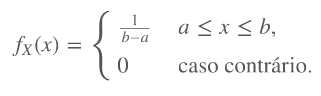
\includegraphics[width=0.5\linewidth]{imagens/eq}
		\caption{Distribuição Uniforme}
		\label{fig:eq}
	\end{figure}
	
	\textbf{Notação:} $X \sim U[a,b]$ ou $X \sim U(a,b)$
	
\subsubsection{Distribuição Acumulada}
	\begin{figure}[h]
		\centering
		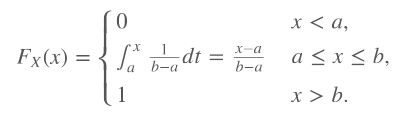
\includegraphics[width=0.5\linewidth]{imagens/eq2}
		\caption{Distribuição Acumulada}
		\label{fig:eq2}
	\end{figure}

\subsubsection{Esperança e Variância}
	\begin{center}
		\Large
		$
		E(X) = \frac{(a + b )}{2}
		$\\
		$
		Var(X) = \frac{(b-a)^2}{12}
		$
	\end{center}
	
\subsection{Distribuição Exponencial}
	Uma v.a X possui distribuição exponencial com parâmetro $\lambda (\lambda>0)$
	\newpage
	\begin{figure}[h]
		\centering
		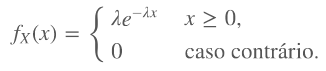
\includegraphics[width=0.5\linewidth]{imagens/eq4}
		\caption{Distribuição Exponencial}
		\label{fig:eq4}
	\end{figure}
	\textbf{Notação:} $X \sim Exp(\lambda)$
	
\subsubsection{Distribuição Acumulada}
	\begin{figure}[h]
		\centering
		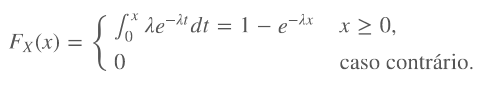
\includegraphics[width=0.5\linewidth]{imagens/eq5}
		\caption{Distribuição Acumulada}
		\label{fig:eq5}
	\end{figure}
	
\subsubsection{Esperança e Variância}
	\begin{center}
		\Large
		$
		E(X) = \frac{1}{\lambda}
		$\\
		$Var(X) = \frac{1}{\lambda ^2}$
	\end{center}

\subsection{Distribuição Normal - Gaussiana}	
	Uma v.a X possui distribuição normal com parâmetros $\mu$ e $\sigma ^2$ se:
	\begin{center}
		\Large	
		$
		f_{x}(x) = \frac{1}{\sqrt{2\pi \sigma ^2}}exp[-\frac{(x-\mu)^2}{2\sigma ^2}]
		$, $
		-\infty<x<\infty
		$
	\end{center}
	\textbf{Notação:} $X \sim N(\mu, \sigma^2)$

\subsubsection{Esperança e Variância}
	\begin{center}
		\Large
		$
		E(X) = \mu
		$\\
		$
		Var(X) = \sigma^2
		$
	\end{center}

\subsubsection{Distribuição Normal Padrão}
	Se $X \sim N(\mu, \sigma^2)$\\
	\begin{center}
		\Large
		$
		Z = \frac{x-\mu}{\sigma}
		$ $\sim N(0,1)$
	\end{center}
	
\subsubsection{Simetria da Distribuição Normal}
	A distribuição normal é simétrica, portanto:
	\begin{center}
		\Large
		$
		P(Z < -z) = P(Z > z)
		$
	\end{center}
	Além disso, temos a seguinte propriedade para a função de distribuição acumulada:
	\begin{center}
		\Large
		$
		\phi (x) = 1 - \phi (-x)
		$
	\end{center}
 	A probabilidade de um intervalo é dada por:
 	\begin{center}
 		\Large
 		$
 		P(a<Z<b) = \phi (b) - \phi (a)
 		$
 	\end{center}
	Onde $\phi (x)$ é a função de densidade acumulada e é encontrada a partir da tabela normal.
	\begin{figure}[h]
		\centering
		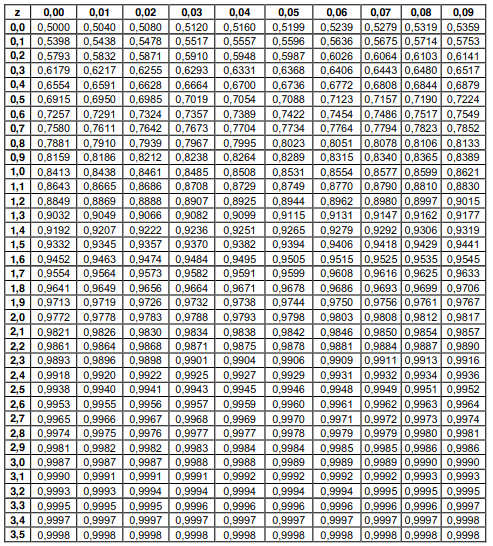
\includegraphics[width=0.9\linewidth]{imagens/tabelaNormal}
		\caption{Tabela para encontrar phi}
		\label{fig:tabelanormal}
	\end{figure}
	
\subsection{Aproximação Normal para uma Binomial}
	Seja $X \sim Bin(n,p)$. Se \textbf{n} é suficientemente grande, a distribuição de X pode ser aproximada pela distribuição normal, isto é:
	\begin{center}
		\Large
		$
		X \sim N(np,np(1-p))
		$
	\end{center}
	Em geral, para que a aproximação para a normal seja utilizada:
	\begin{center}
		\Large
		$
		np\geq 10
		$\\
		$
		n(1-p)\geq 10
		$
	\end{center}
	
\section{Distribuição Amostral}
	Para uma amostra de tamanho \textbf{n} a partir de uma população:
	\begin{itemize}
		\item Com média $\mu$ e variância $\sigma^2$:\\
		$\bar{X}$: $E(\bar{X}) = \mu$ e $Var(\bar{X}) = \frac{\sigma^2}{n}$\\
		Erro Padrão: $EP(\bar{X}) = \sqrt{Var(\bar{X})} = \frac{\sigma}{\sqrt{n}}$
		
		
		\item Com proporção populacional \textit{p}\\
		$\hat{p}$: $E(\hat{p}) = p$ e $Var(\hat{p}) = \frac{p(1-p)}{n}$\\
		Erro Padrão: $EP(\hat{p})=\sqrt{Var(\hat{p})}=\sqrt{\frac{p(1-p)}{n}}$
	\end{itemize}

\subsection{Teorema do Limite Central}
	Para uma amostra aleatória $X_1, ..., X_n$ coletada de uma população com média $\mu$ e variância $\sigma$.\\
	
	A distribuição amostral de $\bar{X}$ aproxima-se de uma \textit{Distribuição Normal} de média $\mu$ e variância $\frac{\sigma^2}{2}$, quando \textbf{n} for suficientemente grande:
	
	\begin{figure}[h]
		\centering
		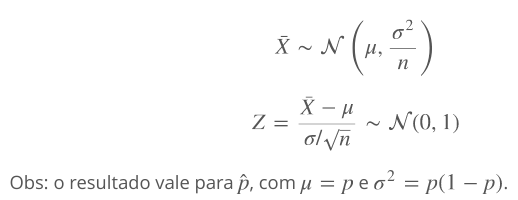
\includegraphics[width=0.7\linewidth]{imagens/teo1}
		\caption{Teorema do Limite Central}
		\label{fig:teo1}
	\end{figure}
	\newpage
	\begin{figure}[h]
		\centering
		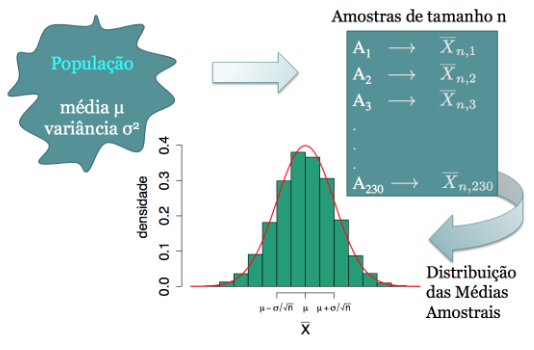
\includegraphics[width=0.7\linewidth]{imagens/teo}
		\caption{Teorema do Limite Central}
		\label{fig:teo}
	\end{figure}
	
\section{Intervalo de Confiança}	
\subsection{Intervalo de Confiança para p}
	Os intervalos de $100(1- \alpha)\%$ de confiança para \textit{p} podem ser de duas formas:
	
	\begin{enumerate}
		\item Método Conservador
			\begin{center}
				\Large
				$
				IC_1(p, 1-\alpha) = [\hat{p} - z_{\alpha /2}\sqrt{\frac{1}{4n}};\hat{p} + z_{\alpha /2}\sqrt{\frac{1}{4n}}] 
				$
			\end{center}
		\item Usando $\hat{p}$ para estimar o erro padrão
			\begin{center}
				\Large
				$
				IC_2(p, 1-\alpha) = [\hat{p} - z_{\alpha /2}\sqrt{\frac{\hat{p}(1-\hat{p})}{n}};\hat{p} + z_{\alpha /2}\sqrt{\frac{\hat{p}(1-\hat{p})}{n}}] 
				$
			\end{center}
	\end{enumerate}

	Veja que nos dois casos, os IC's são da forma $\hat{p}\pm$ margem de erro.
	
\subsubsection{Como encontrar $z_{\alpha/2}$?}
	\begin{center}
		\Large
		$
		1-\alpha = P(|Z| \leq z_{\alpha /2}) = P(-z_{\alpha /2} \leq Z \leq z_{\alpha /2}) = 2\phi (z_{\alpha /2}) -1
		$\\ Portanto,\\
		$
		\phi (z_{\alpha /2}) = 1 - \frac{\alpha}{2} 
		$
	\end{center}
	Procure na tabela o valor de \textit{z} tal que a probabilidade acumulada até o valor de \textit{z} seja $1-\alpha /2$.

\newpage
\subsubsection{Interpretação do Intervalo de Confiança}
	Se várias amostras aleatórias forem retiradas da população e calcularmos um IC de 95\% para cada amostra, cerca de 95\% desses intervalos irão conter a verdadeira proporção na população, p.
	\begin{figure}[h]
		\centering
		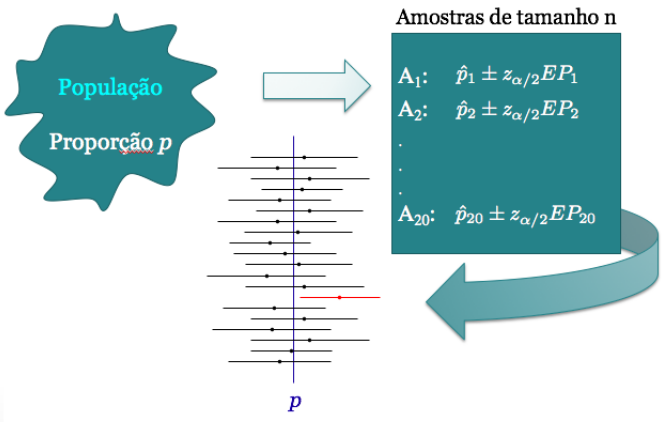
\includegraphics[width=0.7\linewidth]{imagens/ic}
		\caption{Interpretação IC}
		\label{fig:ic}
	\end{figure}
	
\subsubsection{Tamanho da Amostra para Estimar p}
	Em geral, para uma margem de erro \textbf{m}
	\begin{center}
		\Large
		$
		n = (\frac{z_{\alpha /2}}{2m})^2
		$
	\end{center}

\subsection{Intervalo de Confiança para a média populacional $\mu$}
	Seja $X_1, ..., X_n$ uma a.a de uma população com média $\mu$ e variância $ \sigma ^2 $ conhecida. Então:
	\begin{center}
		\Large
		$ 
		Z = \frac{\bar{X}_n - \mu}{\sigma \sqrt{n}}\sim N(0,1)
		$\\
		$ 
		P(-z_{\alpha /2} < Z < z_{\alpha /2}) = 1 - \alpha
		$
	\end{center}
	Um intervalo de $ 100(1-\alpha)\% $ de confiança para $ mu $ é dado por:
	\begin{center}
		\Large
		$ 
		IC(\mu, 1-\alpha) = [\bar{x} - z_{\alpha /2}.\frac{\sigma}{\sqrt{n}}; \bar{x}+z_{\alpha /2}.\frac{\sigma}{\sqrt{n}}]
		$
	\end{center}

\subsubsection{Interpretação do Intervalo de Confiança para $ \mu $}
Imagine que seja possível coletar uma amostra de tamanho \textit{n} da população várias vezes. Para cada vez, você calcula $\bar{a}$ e constrói um IC de 95\% para $\mu$.Imagine também que você conhece $\mu$ e conte quantos dos intervalos contêm $\mu$. A proporção de intervalos que contêm $\mu$ será próxima a 0.95.

\subsubsection{Tamanho da Amostra}
	Em geral, para uma margem de erro \textit{m} e confiança $ 100(1-\alpha) \%$
	\begin{center}
		\Large
		$ 
		n = (\frac{z_{\alpha /2}}{m})^2\sigma ^2
		$
	\end{center}

\subsubsection{Interpretação do Intervalo de Confiança para $ \mu $: $ \sigma$ desconhecido }
	Neste caso, usaremos a variância amostral($ s^2 $) como uma estimativa de $ \sigma ^2 $:
	\begin{center}
		\Large
		$ 
		s^2 = \frac{1}{n - 1} \sum_{i = 1}^{n}(x_i-\bar{x})^2
		$
	\end{center}
	Como consequência, não temos mais distribuição Normal, mas sim a distribuição t-student com n-1 graus de liberdade:
	
	\begin{center}
		\Large
		$ 
		T = \frac{\bar{X}_n - \mu}{\sqrt{s^2/n}} \sim t_n-1
		$\\
		$ 
		P(-t_{n-1, \alpha /2}< T < t_{n-1, \alpha /2}) = 1- \alpha
		$
	\end{center}
	Um intervalo de $ 100(1- \alpha) \%$ de confiança para $\mu$ é dado por:
	\begin{center}
		\Large
		$ 
		IC(\mu, 1- \alpha) = [\bar{x} - t_{n-1, \alpha /2}.\frac{s}{\sqrt{n}};\bar{x} + t_{n-1, \alpha /2}.\frac{s}{\sqrt{n}}]
		$
	\end{center}
	Os valores da distribuição t-student também encontram-se tabelados.

\section{Teste de Hipóteses}
	\begin{enumerate}
		\item Suposições\\
		O teste é válido sob algumas suposições. A mais importante assume que os dados foram coletados aleatoriamente;
		
		\item Hipóteses
			\begin{itemize}
				\item \textbf{Hipótese Nula($H_0$)} afirma que o parâmetro populacional assume um dado valor;
				\item Hipótese \textbf{Alternativa($H_A$)} afirma que o parâmetro populacional assume outros valore, diferente do valor descrito na $H_0$.
			\end{itemize}
		Em testes de hipóteses, mantêm-se a favor de $H_0$ a menos que os dados tragam grande evidência contra.
		
		\item Estatística do Teste\\
		Descreve quão longe do parâmetro populacional usado na $H_0$ a estimativa está;
		
		\item Valor-de-p\\
		Para interpretar uma estatística do teste, vamos usar uma probabilidade para resumir a evidência contra $H_0$, chamada valor-de-p;
		
		\item Conclusão\\
		Geralmente, fixamos o \textbf{nível de significância} do teste($\alpha$), e usamos a seguinte regra - é comum usarmos $\alpha$ = 0,05.
			\begin{itemize}
				\item[$\checkmark$] valor-de-p $< \alpha$: rejeitamos $H_0$
				\item[$\checkmark$] valor-de-p $> \alpha$: não rejeitamos $H_0$
			\end{itemize} 
	\end{enumerate}
\subsubsection{Valor-de-p}
	\begin{figure}[h]
		\centering
		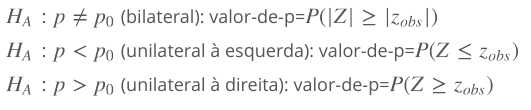
\includegraphics[width=0.7\linewidth]{imagens/p}
		\caption{Valor de p}
		\label{fig:p}
	\end{figure}

\subsubsection{Estatística do Teste}
	Baseada na distribuição amostral de $\hat{p}$.
	\begin{center}
		\Large
		$
		Z = \frac{\hat{p}-p_0}{\sqrt{\frac{p_0(1-p_0)}{n}}}
		$,
		$\sim N(0,1)$
	\end{center}
	
\subsection{Teste de Hipóteses para a média $\sigma$ conhecido}
	Usamos o mesmo passo a passo que foi feito para as proporções:
		\begin{itemize}
			\item Suposições;
			\item Hipóteses;
			\item Estatística do teste:\\
				$
				Z = \frac{\bar{X}-\mu_0}{\frac{\sigma}{\sqrt{n}}}\sim N(0, 1)
				$
			\item Valor-de-p
		\end{itemize}
	
\subsubsection{Região Crítica}
	Conjunto de valores da estatística do teste para as quais a hipótese nula é rejeitada.
	\begin{figure}[h]
		\centering
		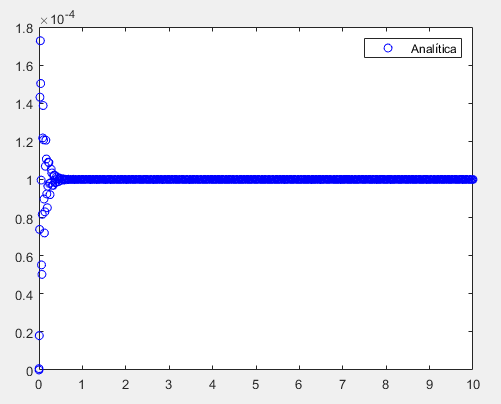
\includegraphics[width=0.8\linewidth]{imagens/g}
		\caption{Região Crítica}
		\label{fig:g}
	\end{figure}
	
\subsection{Teste de Hipóteses para média($\sigma$ desconhecido)}
	Quando $\sigma$ é desconhecido e a amostra é pequena ($n<30$) devemos utilizar a distribuição t.
	\begin{center}
		\Large
		$
		t = \frac{\bar{X}-\mu_0}{\frac{s}{\sqrt{n}}}\sim t_{n-1}
		$
	\end{center}
	Valor-de-p: $P(\mid t_{n-1}\mid \geq \mid t_{obs} \mid ) = 2 p(t_{n-1}\geq t_{obs})$
	
\section{Inferência para duas populações }
\subsection{Intervalo de Confiança para Duas Médias}
	\textbf{Caso 1:} Variâncias diferentes e conhecidas
	\begin{center}
		\Large
		$
		\bar{X} - \bar{Y} \sim N(\mu_1 - \mu_2, \frac{\sigma^2_1}{n} + \frac{\sigma^2_2}{m})
		$
	\end{center}
	
	Normalizando,
	\begin{center}
		\Large
		$
		Z = \frac{(\bar{X} - \bar{Y})-(\mu_1 - \mu_2)}{\sqrt{\frac{\sigma^2_1}{n} + \frac{\sigma^2_2}{m}}} \sim N(0,1)
		$
	\end{center}

	Intervalo de Confiança
	\begin{center}
		\Large
		$
		IC(\mu_1 - \mu_2, 1 - \alpha) = (\bar{X} - \bar{Y}) \pm z_{\frac{\alpha}{2}}\sqrt{\frac{\sigma^2_1}{n} + \frac{\sigma^2_2}{m}}
		$
	\end{center}
	
	\textbf{Caso 2:} Variâncias iguais e conhecidas\\
	É um caso particular em que as variâncias são conhecidas e idênticas, isto é, $\sigma^2_1 = \sigma^2_2 = \sigma^2$\\
	
	\textbf{Caso 3:} Variâncias iguais e desconhecidas\\
	Usamos uma estimativa de $\sigma^2$ e a distribuição normal é substituída pela \textit{distribuição t}.
		\begin{center}
			\Large
			$
			Sp^2 = \frac{(n-1)S^2_1 + (m-1)S^2_2}{n+m-2}
			$\\
			$
			T = \frac{(\bar{X} - \bar{Y})-(\mu_1 - \mu_2)}{\sqrt{Sp^2(\frac{1}{n} + \frac{1}{m})}} \sim t_{n+m-2}
			$\\
			$
			IC(\mu_1 - \mu_2, 1 - \alpha) = (\bar{X} - \bar{Y}) \pm t_{n+m-2}\sqrt{Sp^2(\frac{1}{n} + \frac{1}{m})}
			$
			
		\end{center}
	
\subsection{Intervalo de Confiança para Duas Proporções}
	Queremos encontrar um IC de confiança para a diferença entre as proporções $p_1$ e $p_2$ , ou seja, um IC para $p_1-p_2$.\\
		
		Normalizando,
		\begin{center}
			\Large
			$
			Z = \frac{(\hat{p}_1 - \hat{p}_2)-(p_1-p_2)}{\sqrt{\frac{\hat{p}_1(1-\hat{p_1})}{n_1} + \frac{\hat{p}_2(1-\hat{p_2})}{n_2}}}
			$
		\end{center}
	
		Intervalo de Confiança é dado por:
			\begin{center}
				\Large
				$
				IC(p_1-p_2, 1-\alpha) = (\hat{p}_1 - \hat{p}_2) \pm z_{\frac{\alpha}{2}}\sqrt{\frac{\hat{p}_1(1-\hat{p_1})}{n_1} + \frac{\hat{p}_2(1-\hat{p_2})}{n_2}}
				$
			\end{center}

\subsection{Teste de Hipóteses para duas médias}
	\textbf{Caso 1:} Variâncias diferentes e conhecias\\
	Temos interesse em testar as hipóteses
		\begin{center}
			\Large
			$
			H_0: \mu_1 - \mu_2 = \Delta_0 
			$\\VS\\
			$
			H_A: \mu_1 - \mu_2 \neq \Delta_0 
			$\\
			$
			H_A: \mu_1 - \mu_2 < \Delta_0 
			$\\
			$
			H_A: \mu_1 - \mu_2 > \Delta_0 
			$
		\end{center}
	\textbf{Estatística do Teste}
		\begin{center}
			\Large
			$
			z_{obs} = \frac{(\bar{X} - \bar{Y}) - (\mu_1-\mu_2)}{\sqrt{\frac{\sigma^2_1}{n} + \frac{\sigma^2_2}{m}}} \sim N(0, 1)
			$
		\end{center}
	Depois de calcular a Estatística do Teste, o próximo passo é calcular o \textit{valor-de-p} e comparar com o nível de significância.\\
	
	\textbf{Caso 3:} Variâncias iguais e desconhecidas\\
		\begin{center}
			\Large
			$
			Sp^2 = \frac{(n-1)S^2_1 + (m-1)S^2_2}{n+m-2}
			$
		\end{center}
	Prosseguir usando \textbf{t de student}
\subsection{Teste de Hipóteses para Duas Proporções}
	Considere $X_1, ..., X_{n1}$ e $Y_1, ..., Y_{n1}$ duas amostras independentes de ensaios de Bernoulli tal que $X \sim b(p_1)$ e $Y \sim b(p_2)$, com probabilidade $p_1$ e $p_2$ de apresentarem uma certa característica.
	
		\begin{center}
			\Large
			
			$
			H_0: p_1 - p_2 = 0 
			$\\VS\\
			$
			H_A: p_1 - p_2 \neq 0 
			$\\
			$
			H_A: p_1 - p_2 < 0 
			$\\
			$
			H_A: p_1 - p_2 > 0 
			$\\
			
			Para calcular a estatística do teste precisamos de:\\
			$
			\hat{p} = \frac{n_1\hat{p}_1 + n_2\hat{p_2}}{n_1 + n_2}
			$
			
		\end{center} 
	\textbf{Estatística do Teste}
		\begin{center}
			\Large
			$
			z = \frac{\hat{p}_1 - \hat{p}_2}{\sqrt{\hat{p}(1-\hat{p})(\frac{1}{n_1}+\frac{1}{n_2})}}\sim N(0, 1)
			$
		\end{center}
		








	
\end{document}
